\subsection{Visualization Tools}\label{sec:visualization}
    While analytical approach may provide all necessary information to conduct a technical review of a control system, it might be convenient to present the behavior of the spacecraft in visual form. In these chapters three software solutions are described: one directly implemented in \ac{scars} Toolbox and other two can use simulation outputs to show how modelled satellite performs.
    
    \subsubsection{MATLAB Virtual Reallity Toolbox}
        Virtual Reality Toolbox is an extension for MATLAB which allows creating and interacting with 3D virtual reality models of dynamic systems. In its core it uses \ac{vrml}, a language created in the early days of \ac{www} to display 3D objects and animations. This toolbox provides a way for implementing the \ac{vrml} models inside MATLAB script or Simulink simulation, and allows for control of driving display or animation with MATLAB variables and Simulink signals. Moreover, the toolbox is integrated with \ac{vrml} viewer and \ac{vrml} editor, allowing for building and displaying models directly from MATLAB environment.

        Virtual Reality Toolbox was used in \ac{scars} as most core method of visualization. The \ac{vrml} model is set up with 3 objects: Satellite, Earth and Sun, as they can be considered most useful when observing the effects of the simulation. Satellite model also includes objects representing antennas' range or optical instrument's field of view, if set up in simulation. This feature can be useful for analysis of imaging capabilities.

        The transformations required to process the data generated by \ac{scars}' Vehicle Dynamics block into \ac{vrml} parameters are as follows:
        
        \begin{equation}
            \mathbf{r_{VRML}}=
            \begin{bmatrix}
            1&0&0\\ 
            0&0&-1\\ 
            0&1&0
            \end{bmatrix}
            \mathbf{r_{ECEF}}
        \end{equation}
        
        To calculate spacecraft's rotation vector $\textbf{rot}$ as required by VRML, one has to transform ECEF to Body direction cosine matrix into quaternion $[q_0\: q_1\: q_2\: q_3]$ (scalar first) and then use the following equation:

        \begin{equation}
            \textbf{rot}=
            \begin{bmatrix}
                q_3\\
                q_1\\
                q_0\\
                2*acos(-q_2)
            \end{bmatrix}^T
        \end{equation}

        \autoref{fig:vrml} the example of Virtual World visualization is provided. The animation is set up so that the user can move the camera around, or they can choose (visible in top-left corner) a "Sat Cam" viewpoint, which follows the satellite translation and rotation.

        \begin{figure}[H]
            \centering
            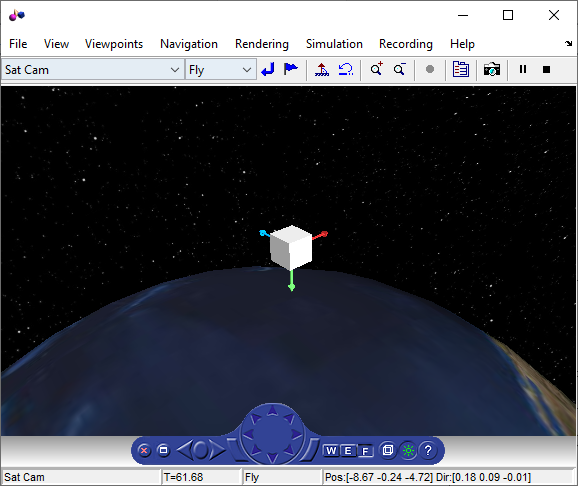
\includegraphics[width=1\textwidth, height=280px]{2-toolbox/vrml.png}
            \caption{Example of Virtual World satellite visualization}
            \label{fig:vrml}
        \end{figure}
        

    \subsubsection{Systems Tool Kit}
        \ac{stk}, formerly named Satellite Tool Kit, is a platform for analyzing and visualizing variety of ground, sea and space platforms missions. \ac{stk} is a commercial software solution used by most major organizations and companies such as \ac{nasa}, \ac{esa}, \ac{dlr}, Boeing, ICEYE. Features most relevant to the topic of this thesis are the graphical engine allowing for displaying the position and attitude of the satellite, and the set of analytical tools, such as ground station connection time calculator, allowing for fine-tuning of mission details.

        To visualize \ac{scars} simulation results with \ac{stk}, one must generate timestamped ephemeris and attitude files. \ac{scars} can generate such files for the user, with predetermined format according to \ac{stk} documentation\cite{stkephemeris}. Both files contain the preamble specifying parameters such as scenario epoch time, central body, coordinate system, distance unit and format of the file. As \ac{scars} relies mostly on \ac{ecef} reference frame, it is also chosen for ephemeris and attitude files. After the preamble, the file contains the lines for each data point. In case of ephemeris file  (\verb|.e| file) the have a format of:

        \begin{Verbatim}[fontsize=\small]
<TimeInSeconds> <X> <Y> <Z> <xDot> <yDot> <zDot>
        \end{Verbatim}

        Where the unit of time is seconds and relative to defined scenario epoch and following parameters are \ac{ecef} vectors in $m$, $m/s$ and $m/s^2$ respectively. For the attitude file (\verb|.a| file), the format is:
        
        \begin{Verbatim}[fontsize=\small]
<TimeInSeconds> <Y> <P> <R>
        \end{Verbatim}
        
        Where time is formatted in same manner as in ephemeris file and the following parameters consist of yaw, pitch and roll Euler angles given in degrees.

        Example \verb|.e| and \verb|.a| files can be found in \autoref{app:efile} and \autoref{app:afile} respectively.

        %https://help.agi.com/stk/11.0.1/Content/stk/importfiles-02.htm#timePosVelAcc

        \begin{figure}[H]
            \centering
            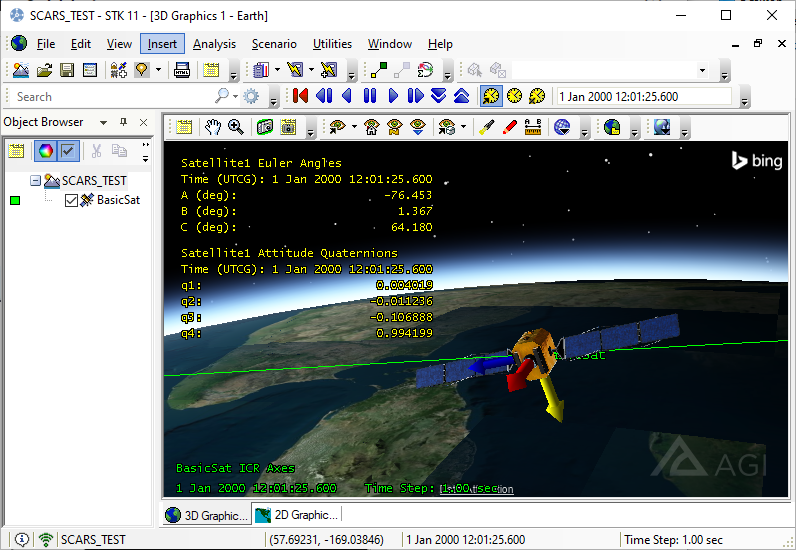
\includegraphics[width=1\textwidth]{2-toolbox/stk_3d.png}
            \caption{Example of STK 3D satellite visualization}
            \label{fig:stk-3d}
        \end{figure}

        \begin{figure}[H]
            \centering
            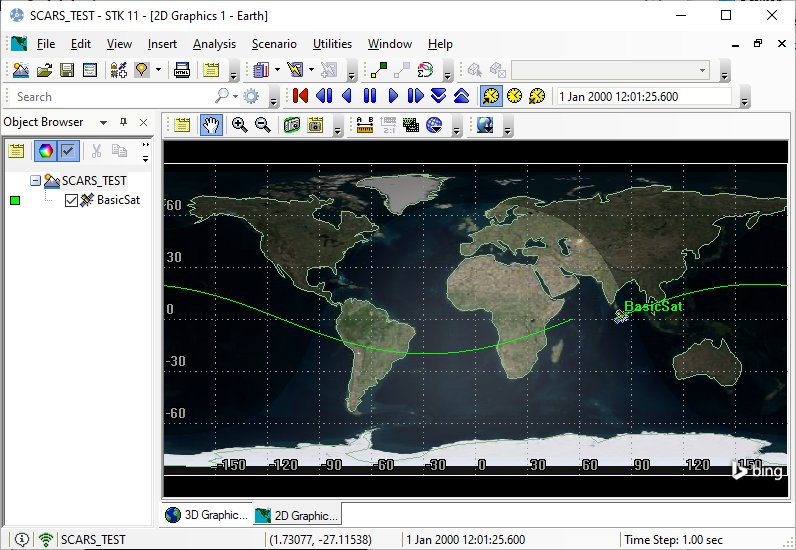
\includegraphics[width=1\textwidth, height=280px]{2-toolbox/stk_groundtrack.png}
            \caption{Example of STK ground track representation}
            \label{fig:stk-ground}
        \end{figure}

        Data produced by a simulation of a simple model, consisting only of \textbf{Environment} and \textbf{Satellite Dynamics} blocks created with SCARS Toolbox was exported into  \verb|.e| and \verb|.a|, from which first lines are shown in mentioned Appendixes. The results were imported into \ac{stk} and can be seen on \autoref{fig:stk-3d} and \autoref{fig:stk-ground}.


    \subsubsection{Kerbal Space Program}\label{sec:ksp}
        Finally, \ac{ksp}, a space flight simulation video game, can be used as a nonconventional method to visualize the results of \ac{scars} Toolbox simulation. In \ac{ksp} the player directs a developing space program originated on fictional Earth-like planet Kerbin. The game provides the tools for the players to design and fly rockets, probes, satellites, spaceplanes, rovers, and other spacecraft from a library of components\cite{kerbals}. The aim of this visualization method was to build a sample satellite in \ac{ksp}, simulate it in \ac{scars} and execute a Hohmann Transfer within a game, using simulation outputs as game inputs.

        The connection between MATLAB and \ac{ksp} is possible because of fanmade \ac{krpc} mod. It creates a API server running alongside the game, with which calls can be made using already written clients in most popular languages, like C++, Python, Lua, Java, etc. Integrating it with MATLAB has proved to be a difficult task, as MATLAB doesn't provide simple means for threading, which means that inputs for the game have to be precalculated to work in real time. Moreover, there is no \ac{krpc} library written directly for MATLAB, therefore a simple Python bridge was written to parse the data taken from the game, compare them with pre-generated \ac{scars} simulation scenario outputs and send them to \ac{ksp} as in-game \ac{aocs} subsystem inputs.

        % \begin{figure}[H]
        %     \centering
        %     \includegraphics[width=1\textwidth, height=100px]{example-image-b}
        %     \caption{Example of kRPC Python client code}
        %     \label{fig:krcp}
        % \end{figure}

        % \dots\textit{rest description and screenshots of visualization}\dots